\documentclass[11pt]{article}

% Language setting
\usepackage[turkish]{babel}
\usepackage{pythonhighlight}

\usepackage[a4paper,top=2cm,bottom=2cm,left=2cm,right=2cm,marginparwidth=2cm]{geometry}

% Useful packages
\usepackage{amsmath}
\usepackage{graphicx}
\usepackage[colorlinks=true, allcolors=blue]{hyperref}
\usepackage{verbatim}
\usepackage{fancyhdr} % for header and footer
\usepackage{titlesec}
\usepackage{parskip}

\setlength{\parindent}{0pt}

\titleformat{\subsection}[runin]{\bfseries}{\thesubsection}{1em}{}

\pagestyle{fancy} % activate the custom header/footer

% define the header/footer contents
\lhead{\small{23BLM-4014 Yapay Sinir Ağları Ara Sınav Soru ve Cevap Kağıdı}}
\rhead{\small{Dr. Ulya Bayram}}
\lfoot{}
\rfoot{}

% remove header/footer on first page
\fancypagestyle{firstpage}{
  \lhead{}
  \rhead{}
  \lfoot{}
  \rfoot{\thepage}
}
 

\title{Çanakkale Onsekiz Mart Üniversitesi, Mühendislik Fakültesi, Bilgisayar Mühendisliği Akademik Dönem 2022-2023\\
Ders: BLM-4014 Yapay Sinir Ağları/Bahar Dönemi\\ 
ARA SINAV SORU VE CEVAP KAĞIDI\\
Dersi Veren Öğretim Elemanı: Dr. Öğretim Üyesi Ulya Bayram}
\author{%
\begin{minipage}{\textwidth}
\raggedright
Öğrenci Adı Soyadı: Umutcan Cerlet\\ % Adınızı soyadınızı ve öğrenci numaranızı noktaların yerine yazın
Öğrenci No: 170401060
\end{minipage}%
}

\date{14 Nisan 2023}

\begin{document}
\maketitle

\vspace{-.5in}
\section*{Açıklamalar:}
\begin{itemize}
    \item Vizeyi çözüp, üzerinde aynı sorular, sizin cevaplar ve sonuçlar olan versiyonunu bu formatta PDF olarak, Teams üzerinden açtığım assignment kısmına yüklemeniz gerekiyor. Bu bahsi geçen PDF'i oluşturmak için LaTeX kullandıysanız, tex dosyasının da yer aldığı Github linkini de ödevin en başına (aşağı url olarak) eklerseniz bonus 5 Puan! (Tavsiye: Overleaf)
    \item Çözümlerde ya da çözümlerin kontrolünü yapmada internetten faydalanmak, ChatGPT gibi servisleri kullanmak serbest. Fakat, herkesin çözümü kendi emeğinden oluşmak zorunda. Çözümlerinizi, cevaplarınızı aşağıda belirttiğim tarih ve saate kadar kimseyle paylaşmayınız. 
    \item Kopyayı önlemek için Github repository'lerinizin hiçbirini \textbf{14 Nisan 2023, saat 15:00'a kadar halka açık (public) yapmayınız!} (Assignment son yükleme saati 13:00 ama internet bağlantısı sorunları olabilir diye en fazla ekstra 2 saat daha vaktiniz var. \textbf{Fakat 13:00 - 15:00 arası yüklemelerden -5 puan!}
    \item Ek puan almak için sağlayacağınız tüm Github repository'lerini \textbf{en geç 15 Nisan 2023 15:00'da halka açık (public) yapmış olun linklerden puan alabilmek için!}
    \item \textbf{14 Nisan 2023, saat 15:00'dan sonra gönderilen vizeler değerlendirilmeye alınmayacak, vize notu olarak 0 (sıfır) verilecektir!} Son anda internet bağlantısı gibi sebeplerden sıfır almayı önlemek için assignment kısmından ara ara çözümlerinizi yükleyebilirsiniz yedekleme için. Verilen son tarih/saatte (14 Nisan 2023, saat 15:00) sistemdeki en son yüklü PDF geçerli olacak.
    \item Çözümlerin ve kodların size ait ve özgün olup olmadığını kontrol eden bir algoritma kullanılacaktır. Kopya çektiği belirlenen vizeler otomatikman 0 (sıfır) alacaktır. Bu nedenle çözümlerinizi ve kodlarınızı yukarıda sağladığım gün ve saatlere kadar kimseyle paylaşmayınız.
    \item Bu vizeden alınabilecek en yüksek not 100'dür. Toplam aldığınız puan 100'ü geçerse, aldığınız not 100'e sabitlenecektir.
    \item LaTeX kullanarak PDF oluşturanlar öz geçmişlerine LaTeX bildiklerini de eklemeyi unutmasınlar :)
    \item Bu vizedeki soruların çözümleri ve tex dosyası için istediğiniz kadar sayıda Github repository'si oluşturabilirsiniz. Sadece yukarıda belirttiğim tarihlerde (14 Nisan 2023 saat 15:00 ile 15 Nisan 2023 saat 15:00 arasında) public yapmayı/halka açmayı ve Github profilinizi de öz geçmişinize eklemeyi unutmayın :)
    \item Bilgisayarınıza hiçbir program kurmadan, Overleaf, Google Colab, Kaggle gibi ortamlar üzerinden bu vizeyi tamamlamanız mümkün. İyi çalışmalar!!
\end{itemize}

(Ekstra 5 puan) \url{OdevinTexDosyasınınGithubLinkiniburayakoyun.com}

\newpage
\section{(Toplam 10 Puan) Hopfield Networks:}

\subsection{(2 Puan)} \textbf{ChatGPT’ye size Hopfield Network’ler ile ilgili detaylı bilgi vermesini isteyin. Sorduğunuz soruyu, ChatGPT'nin çıkartığı cevabı aşağı koyun. Bu cevapta anlamadığınız terimleri de ChatGPT’ye sorup, sorduğunuz soruları ve ChatGPT’nin verdiği cevapları da sırayla aşağı koyun.}

Hopfield Network’ler ile ilgili detaylı bilgi verebilir misin bana?

Elbette! Hopfield ağları, yapay sinir ağları alanında kullanılan bir tür geri beslemeli ve asenkron enerji tabanlı bir modeldir. Yapay sinir ağları, insan beyninin işleyişinden esinlenerek tasarlanan matematiksel modellerdir ve çeşitli uygulamalarda kullanılır. Hopfield ağları, bellek ve hatırlama gibi uygulamalarda kullanılabilir ve özellikle küçük ve orta ölçekli problemleri çözmek için kullanışlıdır.

Hopfield ağları, asenkron dinamiklere sahip bir enerji fonksiyonu ile tanımlanır ve her bir nöron, tüm diğer nöronlarla bağlantılıdır. Hopfield ağları, bir nöronun durumunu diğer nöronların durumlarından türeterek çalışır ve ağdaki nöronların etkileşimleri sonucu bir enerji fonksiyonu minimize edilir.

Hopfield ağları, iki temel modda çalışabilir: öğrenme ve hatırlama. Öğrenme aşamasında, ağa hafızada saklanmak istenen desenler verilir ve ağ, bu desenlere göre ağırlıklarını günceller. Hatırlama aşamasında ise, ağa parçalı veya hatalı bir giriş deseni verildiğinde, ağ, giriş desenine en yakın olan saklanmış deseni hatırlayarak tamamlar.

Hopfield ağlarının avantajlarından biri, giriş desenine yakın olan hatırlanmış desenleri hatırlama yetenekleridir. Ayrıca, hafızadaki desenlere gürültü eklenmiş giriş desenlerini hatırlayabilirler ve hatalı desenleri düzeltebilirler. Bununla birlikte, Hopfield ağlarının bellek kapasitesi sınırlıdır ve büyük veri kümesi üzerinde kullanılmak için uygun değildir.

Hopfield ağları, çeşitli uygulamalarda kullanılabilir, özellikle desen tanıma, bellek ve hatırlama, optimize etme gibi problemlerde başarıyla kullanılmıştır. Ancak, büyük veri kümesi üzerinde kullanıldığında sınırlamaları nedeniyle diğer daha karmaşık sinir ağı modelleri tercih edilebilir.


\subsection{(8 Puan)} \textbf{ChatGPT’nin açıklamalarından ne anladığınızı buraya kendi kelimelerinizle özetleyin. Örneğin ``Hopfield Network nedir? Ne işe yarar? Neden bilmemiz gerekir bunu? Gerçek hayatta kullanılıyor mu?'' gibi. Anlamadığınız kısımlar varsa ve ChatGPT’nin açıklamaları yeterli gelmezse internet dahil farklı kaynaklardan araştırıp, bilgilerin doğruluğunu sorgulamakta serbestsiniz. Konuyu doğru anlayıp anlamamanız puana etki edecektir. Kullandığınız kaynakları da belirtin!}

Hopfield ağı çağrışımsal olarak çevirebilen bir modeldir. Bu ağ bir katmana sahiptir. Input ve output katmanları birebir aynı özelliktedir. Bu tür ağlarda nöron sayısı önemlidir. Bu sayıya göre ağın kapasitesi belirlenebilir. İki türlü aşama bulunmaktadır. Bu aşamalar depolama ve geri çağırma aşaması olarak tanımlandırılır.

Depolama(Eğitim): Nesneler ve karakterler depolanabilir.
Hopfield ağının en önemli özelliği; katmandaki nöronların hepsi birbirine bağlıdır.

Kısaca, hopfield ağ modeli, her biri birbirine bağlı nöronlardan oluşan bir kümedir. Girdi ve çıktı kümeleri arasında fark yoktur.

Kullanım alanları;
-Şifreleme işlemlerinde
-Karakter-Desen Eşleştirmede
-Bozuk Şekillerin Yeniden Oluşturulmasında
-El Yazı Tanımlama Sistemlerinde

\url{'https://medium.com/@batincangurbuz/hopfield-a%C4%9F-modeli-hopfield-network-hn-ccf1548ca432'}

\section{(Toplam 10 Puan) Boltzman Machine:}

\subsection{(2 Puan)} \textbf{ChatGPT’ye size Boltzman Machine ilgili detaylı bilgi vermesini isteyin. Sorduğunuz soruyu, ChatGPT'nin çıkartığı cevabı aşağı koyun. Bu cevapta anlamadığınız terimleri de ChatGPT’ye sorup, sorduğunuz soruları ve ChatGPT’nin verdiği cevapları da sırayla aşağı koyun.}

Boltzman Machine ile ilgili detaylı bilgi verir misin?

Elbette! Boltzmann Makinesi (Boltzmann Machine), yapay sinir ağları alanında kullanılan bir tür olasılıksal ve stokastik bir modeldir. Boltzmann Makinesi, enerji tabanlı bir model olarak tanımlanır ve genellikle olasılıksal lojistik fonksiyonları kullanır. Boltzmann Makinesi, kısıtlı bir ağ yapısına ve gizli katmanlara sahip olmayan bir tür olasılıksal bir modeldir.

Boltzmann Makinesi, iki tür nöron içerir: görünür nöronlar ve gizli nöronlar. Görünür nöronlar, ağa doğrudan veri girişini temsil ederken, gizli nöronlar, giriş verilerinin anlamlı özelliklerini öğrenen gizli bir temsil oluşturur. Bu nöronlar arasındaki etkileşim, enerji fonksiyonu denilen bir fonksiyonla tanımlanır. Enerji fonksiyonu, ağın durumlarını enerji seviyeleri aracılığıyla değerlendirir ve ağın hangi durumların daha olası olduğunu belirler.

Boltzmann Makinesi, öğrenme ve yeniden yapılandırma aşamaları olmak üzere iki temel aşamada çalışır. Öğrenme aşamasında, ağa giriş veri örnekleri verilir ve ağ, veriyi modellemek için ağırlıklarını günceller. Yeniden yapılandırma aşamasında ise, ağa başlangıçtaki durum verilerek ağın yeni bir durumunu örnekleme yaparak elde eder.

Boltzmann Makineleri, çeşitli uygulamalarda kullanılabilir, özellikle tahmin, modelleme, veri sıkıştırma ve olasılıksal jenerasyon gibi problemlerde başarıyla kullanılmıştır. Bununla birlikte, Boltzmann Makineleri, yüksek hesaplama gücü gerektirdiği için büyük veri kümesi üzerinde kullanıldığında zaman alabilir ve eğitim süreçleri karmaşık olabilir. Bu nedenle, daha sonraki türetilmiş modelleri, örneğin Hızlı Gizli Durumlar (Restricted Boltzmann Machine, RBM) gibi gelişmiş varyantlarını içerir.

\subsection{(8 Puan)} \textbf{ChatGPT’nin açıklamalarından ne anladığınızı buraya kendi kelimelerinizle özetleyin. Örneğin ``Boltzman Machine nedir? Ne işe yarar? Neden bilmemiz gerekir bunu? Gerçek hayatta kullanılıyor mu?'' gibi. Anlamadığınız kısımlar varsa ve ChatGPT’nin açıklamaları yeterli gelmezse internet dahil farklı kaynaklardan araştırıp, bilgilerin doğruluğunu sorgulamakta serbestsiniz. Konuyu doğru anlayıp anlamamanız puana etki edecektir. Kullandığınız kaynakları da belirtin!}

2006'da ilk kez Geoffrey Hinton tarafından ortaya atılmış bir hızlı öğrenme algoritmasıdır.
Bu algoritmayla sınıflandırma,regression ve featuresların öğrenimi gibi işlemleri yapabiliriz. Aynı zamanda giriş veri setindeki olasılıksal dağılımları öğrenebilecek bir ağdır. Hopfield ağlarının stokastik(sezgiye dayalı) üretken bir karşılığı olarak görülebilir. Pratik bir sonuç beklememek gerekir. Zor kombinasyon problemlerini temsil edip çözebilirler. Input ve hidden layerdaki her nöron benzeri bir nöronu temsil eder. Bu nöronlarda basitçe hesaplamalar gerçekleştirilebilir. En önemli nokta; nöronlar birbirlerine katmanlar halinde bağlanabilir ancak aynı katmandaki iki düğüm birbirine bağlanamaz. Bundan dolayı da katman içi iletişim yoktur.

\url{'https://medium.com/@batincangurbuz/boltzman-makinesi-boltzmann-machines-bm-ve-k%C4%B1s%C4%B1tlanm%C4%B1%C5%9F-boltzmann-makineleri-restricted-boltzmann-6f2e0f839b05'}

\section{(Toplam 10 Puan) Markov Assumption ve Markov Chain:}

\subsection{(2 Puan)} \textbf{ChatGPT’ye size Markov assumption ve Markov Chain ilgili detaylı bilgi vermesini isteyin. Sorduğunuz soruyu, ChatGPT'nin çıkartığı cevabı aşağı koyun. Bu cevapta anlamadığınız terimleri de ChatGPT’ye sorup, sorduğunuz soruları ve ChatGPT’nin verdiği cevapları da sırayla aşağı koyun.}

Markov assumption ve Markov Chain ile ilgili detaylı bilgi verir misin?

Elbette! Markov varsayımı (Markov assumption), bir sürecin gelecekteki durumunu sadece mevcut durumuna bağlı olarak tahmin etme prensibidir. Diğer bir deyişle, bir sürecin gelecekteki durumu, şu anki durumu bilerek tahmin edilebilir ve geçmiş durumlar, gelecekteki durumu etkilemez. Bu varsayım, Markov zinciri (Markov Chain) olarak adlandırılan bir olasılık süreci modelini tanımlar.

Markov zinciri, Markov varsayımını karşılayan bir süreçtir. Bir Markov zinciri, sürecin gelecekteki durumunu, yalnızca şu anki durumuna bağlı olarak tahmin edebildiği bir durum uzayı ile karakterizedir. Markov zinciri, zamana bağlı bir seri olayı modellemek için kullanılabilir, örneğin finans, biyoloji, iletişim ağları, rastgele yürüyüşler ve daha pek çok uygulama alanında kullanılır.

Markov zinciri, genellikle iki temel bileşenden oluşur: durum uzayı ve geçiş olasılıkları. Durum uzayı, sürecin alabileceği tüm durumların kümesidir. Geçiş olasılıkları, bir durumdan başka bir duruma geçişin olasılıklarını belirler. Bu olasılıklar, genellikle geçiş olasılık matrisi veya geçiş olasılık fonksiyonu olarak ifade edilir.

Markov zincirleri, zaman bağımlı bir süreci modellemek için kullanılır ve mevcut duruma dayanarak gelecekteki durumu tahmin etmek için kullanılır. Markov zincirleri, zamanın önemli olduğu, geçmiş durumların gelecekteki durumu etkilediği durumlarda kullanışlıdır. Örneğin, hava durumu tahminleri, finansal piyasa modelleri, doğal dil işleme ve genetik modeller gibi uygulama alanlarında yaygın olarak kullanılır.

Markov zincirleri, zamanla geliştirilen ve geliştirilen bir dizi ileri düzey modelin temelini oluşturur. Örnek olarak, gizli Markov modelleri (Hidden Markov Models, HMM) gibi daha karmaşık Markov zinciri varyantları, girdi verisindeki gizli durumları modellemek için kullanılır. Markov zincirleri, olasılıklı ve zaman bağımlı modellere ilgi duyan istatistikçiler, veri bilimcileri ve mühendisler için önemli bir araçtır.

\subsection{(8 Puan)} \textbf{ChatGPT’nin açıklamalarından ne anladığınızı buraya kendi kelimelerinizle özetleyin. Örneğin ``Markov assumption ve Markov Chain nedir? Ne işe yarar? Neden bilmemiz gerekir bunu? Gerçek hayatta kullanılıyor mu?'' gibi. Anlamadığınız kısımlar varsa ve ChatGPT’nin açıklamaları yeterli gelmezse internet dahil farklı kaynaklardan araştırıp, bilgilerin doğruluğunu sorgulamakta serbestsiniz. Konuyu doğru anlayıp anlamamanız puana etki edecektir. Kullandığınız kaynakları da belirtin!}

Markov zinciri, markov özelliğine sahip bir stokastik süreçtir. Bu özelliğe sahip olmak, mevcut durum verildiğinde gelecek durumların geçmiş durumlardan bağımsız olması anlamına gelir. Gelecek durumlara belirli bir şekilde değil, olasılıksal bir süreçle ulaşılır.

Bir T anında sistem belirli bir olasılık dağlımına bağlı olarak o anki durumundan başka bir duruma geçebilir ya da o anki durumunu koruyabilir.

Markov zincirinin özellikleri;
-İndirgenebilirlik
-Dönemsellik
-Tekrarlama
-Ergodiklik

Çeşitli markov zincirleri literatürde bulunmaktadır. Sequence bir modeldir. Bu model her input olarak verilen sequence'deki her nörona bir çıktı yaratır. Yani her olası çıktı için bir olasılık hesaplar ve en olası olanı seçer.

\url{'https://egealpay1.medium.com/hidden-markov-models-sakl%C4%B1-markov-modeli-b381380d0aca'}

\section{(Toplam 20 Puan) Feed Forward:}
 
\begin{itemize}
    \item Forward propagation için, input olarak şu X matrisini verin (tensöre çevirmeyi unutmayın):\\
    $X = \begin{bmatrix}
        1 & 2 & 3\\
        4 & 5 & 6
        \end{bmatrix}$
    Satırlar veriler (sample'lar), kolonlar öznitelikler (feature'lar).
    \item Bir adet hidden layer olsun ve içinde tanh aktivasyon fonksiyonu olsun
    \item Hidden layer'da 50 nöron olsun
    \item Bir adet output layer olsun, tek nöronu olsun ve içinde sigmoid aktivasyon fonksiyonu olsun
\end{itemize}

Tanh fonksiyonu:\\
$f(x) = \frac{exp(x) - exp(-x)}{exp(x) + exp(-x)}$
\vspace{.2in}

Sigmoid fonksiyonu:\\
$f(x) = \frac{1}{1 + exp(-x)}$

\vspace{.2in}
 \textbf{Pytorch kütüphanesi ile, ama kütüphanenin hazır aktivasyon fonksiyonlarını kullanmadan, formülünü verdiğim iki aktivasyon fonksiyonunun kodunu ikinci haftada yaptığımız gibi kendiniz yazarak bu yapay sinir ağını oluşturun ve aşağıdaki üç soruya cevap verin.}
 
\subsection{(10 Puan)} \textbf{Yukarıdaki yapay sinir ağını çalıştırmadan önce pytorch için Seed değerini 1 olarak set edin, kodu aşağıdaki kod bloğuna ve altına da sonucu yapıştırın:}

% Latex'de kod koyabilirsiniz python formatında. Aşağıdaki örnekleri silip içine kendi kodunuzu koyun
\begin{python}
import torch
import torch.nn.functional as F
import torch.optim as optim

torch.manual_seed(1)

x = torch.tensor([[1,2,3], [4,5,6]], dtype=torch.float32)

# tanh fonksiyonunu pytorch kullanmadan yazdım.
def tanh(x):
    return (torch.exp(x) - torch.exp(-x)) / (torch.exp(x) + torch.exp(-x))

# sigmoid fonksiyonunu pytorch kullanmadan yazdım.
def sigmoid(x):
    return 1 / (1 + torch.exp(-x))

class NeuralNet(torch.nn.Module):
    def __init__(self, input_size, hidden_size, output_size):
        super(NeuralNet, self).__init__()
        self.hidden = torch.nn.Linear(input_size, hidden_size)
        self.output = torch.nn.Linear(hidden_size, output_size)

    def forward(self, x):
        hidden_layer = self.hidden(x)
        activated_hidden_layer = tanh(hidden_layer)
        output_layer = self.output(activated_hidden_layer)
        activated_output_layer = sigmoid(output_layer)
        return activated_output_layer

# Modeli oluştur
input_size = 3
hidden_size = 50
output_size = 1
model = NeuralNet(input_size, hidden_size, output_size)

# Binary cross entropy loss fonksiyonunu tanımla
criterion = F.binary_cross_entropy

# Stochastic gradient descent optimizer'ı tanımla
optimizer = optim.SGD(model.parameters(), lr=0.1)

# Veri setini oluştur
x = torch.tensor([[1,2,3], [4,5,6]], dtype=torch.float32)
y = torch.tensor([0, 1], dtype=torch.float32).reshape(-1, 1)

# Training döngüsü
for epoch in range(100):
    # Tahminleri hesapla
    y_pred = model(x)

    # Loss değerini hesapla ve print et
    loss = criterion(y_pred, y)
    
    print('Epoch {}: Loss = {:.5f}'.format(epoch+1, loss))

    # Gradyanları sıfırla, loss değerine göre gradiyanları hesapla ve optimize et
    optimizer.zero_grad()
    loss.backward()
    optimizer.step()
\end{python}

Epoch 1: Loss = 0.62883
Epoch 2: Loss = 0.59458
Epoch 3: Loss = 0.56336
Epoch 4: Loss = 0.53301
Epoch 5: Loss = 0.50355
Epoch 6: Loss = 0.47523
Epoch 7: Loss = 0.44837
Epoch 8: Loss = 0.42324
Epoch 9: Loss = 0.40001
Epoch 10: Loss = 0.37866
Epoch 11: Loss = 0.35906
Epoch 12: Loss = 0.34101
Epoch 13: Loss = 0.32429
Epoch 14: Loss = 0.30872
Epoch 15: Loss = 0.29417
Epoch 16: Loss = 0.28051
Epoch 17: Loss = 0.26766
Epoch 18: Loss = 0.25554
Epoch 19: Loss = 0.24410
Epoch 20: Loss = 0.23330
Epoch 21: Loss = 0.22310
Epoch 22: Loss = 0.21346
Epoch 23: Loss = 0.20435
Epoch 24: Loss = 0.19575
Epoch 25: Loss = 0.18762
Epoch 26: Loss = 0.17994
Epoch 27: Loss = 0.17269
Epoch 28: Loss = 0.16583
Epoch 29: Loss = 0.15935
Epoch 30: Loss = 0.15322
Epoch 31: Loss = 0.14743
Epoch 32: Loss = 0.14195
Epoch 33: Loss = 0.13676
Epoch 34: Loss = 0.13186
Epoch 35: Loss = 0.12722
Epoch 36: Loss = 0.12283
Epoch 37: Loss = 0.11868
Epoch 38: Loss = 0.11474
Epoch 39: Loss = 0.11101
Epoch 40: Loss = 0.10748
Epoch 41: Loss = 0.10412
Epoch 42: Loss = 0.10094
Epoch 43: Loss = 0.09792
Epoch 44: Loss = 0.09505
Epoch 45: Loss = 0.09232
Epoch 46: Loss = 0.08973
Epoch 47: Loss = 0.08725
Epoch 48: Loss = 0.08490
Epoch 49: Loss = 0.08265
Epoch 50: Loss = 0.08050
Epoch 51: Loss = 0.07845
Epoch 52: Loss = 0.07649
Epoch 53: Loss = 0.07461
Epoch 54: Loss = 0.07282
Epoch 55: Loss = 0.07110
Epoch 56: Loss = 0.06944
Epoch 57: Loss = 0.06786
Epoch 58: Loss = 0.06633
Epoch 59: Loss = 0.06487
Epoch 60: Loss = 0.06346
Epoch 61: Loss = 0.06211
Epoch 62: Loss = 0.06080
Epoch 63: Loss = 0.05955
Epoch 64: Loss = 0.05833
Epoch 65: Loss = 0.05716
Epoch 66: Loss = 0.05603
Epoch 67: Loss = 0.05494
Epoch 68: Loss = 0.05389
Epoch 69: Loss = 0.05287
Epoch 70: Loss = 0.05189
Epoch 71: Loss = 0.05093
Epoch 72: Loss = 0.05001
Epoch 73: Loss = 0.04912
Epoch 74: Loss = 0.04825
Epoch 75: Loss = 0.04741
Epoch 76: Loss = 0.04660
Epoch 77: Loss = 0.04581
Epoch 78: Loss = 0.04504
Epoch 79: Loss = 0.04430
Epoch 80: Loss = 0.04358
Epoch 81: Loss = 0.04288
Epoch 82: Loss = 0.04220
Epoch 83: Loss = 0.04153
Epoch 84: Loss = 0.04089
Epoch 85: Loss = 0.04026
Epoch 86: Loss = 0.03965
Epoch 87: Loss = 0.03906
Epoch 88: Loss = 0.03848
Epoch 89: Loss = 0.03791
Epoch 90: Loss = 0.03736
Epoch 91: Loss = 0.03683
Epoch 92: Loss = 0.03631
Epoch 93: Loss = 0.03580
Epoch 94: Loss = 0.03530
Epoch 95: Loss = 0.03482
Epoch 96: Loss = 0.03435
Epoch 97: Loss = 0.03389
Epoch 98: Loss = 0.03344
Epoch 99: Loss = 0.03300
Epoch 100: Loss = 0.03257

\subsection{(5 Puan)} \textbf{Yukarıdaki yapay sinir ağını çalıştırmadan önce Seed değerini öğrenci numaranız olarak değiştirip, kodu aşağıdaki kod bloğuna ve altına da sonucu yapıştırın:}

\begin{python}
import torch
import torch.nn.functional as F
import torch.optim as optim

torch.manual_seed(170401060)

x = torch.tensor([[1,2,3], [4,5,6]], dtype=torch.float32)

# tanh fonksiyonunu pytorch kullanmadan yazdım.
def tanh(x):
    return (torch.exp(x) - torch.exp(-x)) / (torch.exp(x) + torch.exp(-x))

# sigmoid fonksiyonunu pytorch kullanmadan yazdım.
def sigmoid(x):
    return 1 / (1 + torch.exp(-x))

class NeuralNet(torch.nn.Module):
    def __init__(self, input_size, hidden_size, output_size):
        super(NeuralNet, self).__init__()
        self.hidden = torch.nn.Linear(input_size, hidden_size)
        self.output = torch.nn.Linear(hidden_size, output_size)

    def forward(self, x):
        hidden_layer = self.hidden(x)
        activated_hidden_layer = tanh(hidden_layer)
        output_layer = self.output(activated_hidden_layer)
        activated_output_layer = sigmoid(output_layer)
        return activated_output_layer

# Modeli oluştur
input_size = 3
hidden_size = 50
output_size = 1
model = NeuralNet(input_size, hidden_size, output_size)

# Binary cross entropy loss fonksiyonunu tanımla
criterion = F.binary_cross_entropy

# Stochastic gradient descent optimizer'ı tanımla
optimizer = optim.SGD(model.parameters(), lr=0.1)

# Veri setini oluştur
x = torch.tensor([[1,2,3], [4,5,6]], dtype=torch.float32)
y = torch.tensor([0, 1], dtype=torch.float32).reshape(-1, 1)

# Training döngüsü
for epoch in range(100):
    # Tahminleri hesapla
    y_pred = model(x)

    # Loss değerini hesapla ve print et
    loss = criterion(y_pred, y)
    
    print('Epoch {}: Loss = {:.5f}'.format(epoch+1, loss))

    # Gradyanları sıfırla, loss değerine göre gradiyanları hesapla ve optimize et
    optimizer.zero_grad()
    loss.backward()
    optimizer.step()
\end{python}

Epoch 1: Loss = 0.74455
Epoch 2: Loss = 0.65688
Epoch 3: Loss = 0.63686
Epoch 4: Loss = 0.61787
Epoch 5: Loss = 0.59960
Epoch 6: Loss = 0.58190
Epoch 7: Loss = 0.56466
Epoch 8: Loss = 0.54779
Epoch 9: Loss = 0.53125
Epoch 10: Loss = 0.51504
Epoch 11: Loss = 0.49917
Epoch 12: Loss = 0.48367
Epoch 13: Loss = 0.46857
Epoch 14: Loss = 0.45387
Epoch 15: Loss = 0.43957
Epoch 16: Loss = 0.42566
Epoch 17: Loss = 0.41212
Epoch 18: Loss = 0.39891
Epoch 19: Loss = 0.38603
Epoch 20: Loss = 0.37344
Epoch 21: Loss = 0.36115
Epoch 22: Loss = 0.34913
Epoch 23: Loss = 0.33739
Epoch 24: Loss = 0.32592
Epoch 25: Loss = 0.31472
Epoch 26: Loss = 0.30378
Epoch 27: Loss = 0.29312
Epoch 28: Loss = 0.28272
Epoch 29: Loss = 0.27262
Epoch 30: Loss = 0.26281
Epoch 31: Loss = 0.25333
Epoch 32: Loss = 0.24420
Epoch 33: Loss = 0.23546
Epoch 34: Loss = 0.22712
Epoch 35: Loss = 0.21918
Epoch 36: Loss = 0.21165
Epoch 37: Loss = 0.20450
Epoch 38: Loss = 0.19771
Epoch 39: Loss = 0.19126
Epoch 40: Loss = 0.18512
Epoch 41: Loss = 0.17926
Epoch 42: Loss = 0.17368
Epoch 43: Loss = 0.16834
Epoch 44: Loss = 0.16324
Epoch 45: Loss = 0.15837
Epoch 46: Loss = 0.15369
Epoch 47: Loss = 0.14922
Epoch 48: Loss = 0.14494
Epoch 49: Loss = 0.14083
Epoch 50: Loss = 0.13689
Epoch 51: Loss = 0.13311
Epoch 52: Loss = 0.12949
Epoch 53: Loss = 0.12601
Epoch 54: Loss = 0.12267
Epoch 55: Loss = 0.11947
Epoch 56: Loss = 0.11639
Epoch 57: Loss = 0.11343
Epoch 58: Loss = 0.11059
Epoch 59: Loss = 0.10786
Epoch 60: Loss = 0.10524
Epoch 61: Loss = 0.10271
Epoch 62: Loss = 0.10028
Epoch 63: Loss = 0.09794
Epoch 64: Loss = 0.09569
Epoch 65: Loss = 0.09352
Epoch 66: Loss = 0.09142
Epoch 67: Loss = 0.08941
Epoch 68: Loss = 0.08746
Epoch 69: Loss = 0.08558
Epoch 70: Loss = 0.08377
Epoch 71: Loss = 0.08202
Epoch 72: Loss = 0.08032
Epoch 73: Loss = 0.07869
Epoch 74: Loss = 0.07711
Epoch 75: Loss = 0.07558
Epoch 76: Loss = 0.07409
Epoch 77: Loss = 0.07266
Epoch 78: Loss = 0.07127
Epoch 79: Loss = 0.06993
Epoch 80: Loss = 0.06862
Epoch 81: Loss = 0.06736
Epoch 82: Loss = 0.06613
Epoch 83: Loss = 0.06494
Epoch 84: Loss = 0.06379
Epoch 85: Loss = 0.06267
Epoch 86: Loss = 0.06158
Epoch 87: Loss = 0.06052
Epoch 88: Loss = 0.05950
Epoch 89: Loss = 0.05850
Epoch 90: Loss = 0.05753
Epoch 91: Loss = 0.05658
Epoch 92: Loss = 0.05567
Epoch 93: Loss = 0.05477
Epoch 94: Loss = 0.05390
Epoch 95: Loss = 0.05306
Epoch 96: Loss = 0.05223
Epoch 97: Loss = 0.05143
Epoch 98: Loss = 0.05065
Epoch 99: Loss = 0.04988
Epoch 100: Loss = 0.04914

\subsection{(5 Puan)} \textbf{Kodlarınızın ve sonuçlarınızın olduğu jupyter notebook'un Github repository'sindeki linkini aşağıdaki url kısmının içine yapıştırın. İlk sayfada belirttiğim gün ve saate kadar halka açık (public) olmasın:}
% size ait Github olmak zorunda, bu vize için ayrı bir github repository'si açıp notebook'u onun içine koyun. Kendine ait olmayıp da arkadaşının notebook'unun linkini paylaşanlar 0 alacak.

\url{https://github.com/UmutcanCerlet604/neural_networks_1.git}

\section{(Toplam 40 Puan) Multilayer Perceptron (MLP):} 
\textbf{Bu bölümdeki sorularda benim vize ile beraber paylaştığım Prensesi İyileştir (Cure The Princess) Veri Seti parçaları kullanılacak. Hikaye şöyle (soruyu çözmek için hikaye kısmını okumak zorunda değilsiniz):} 

``Bir zamanlar, çok uzaklarda bir ülkede, ağır bir hastalığa yakalanmış bir prenses yaşarmış. Ülkenin kralı ve kraliçesi onu iyileştirmek için ellerinden gelen her şeyi yapmışlar, ancak denedikleri hiçbir çare işe yaramamış.

Yerel bir grup köylü, herhangi bir hastalığı iyileştirmek için gücü olduğu söylenen bir dizi sihirli malzemeden bahsederek kral ve kraliçeye yaklaşmış. Ancak, köylüler kral ile kraliçeyi, bu malzemelerin etkilerinin patlayıcı olabileceği ve son zamanlarda yaşanan kuraklıklar nedeniyle bu malzemelerden sadece birkaçının herhangi bir zamanda bulunabileceği konusunda uyarmışlar. Ayrıca, sadece deneyimli bir simyacı bu özelliklere sahip patlayıcı ve az bulunan malzemelerin belirli bir kombinasyonunun prensesi iyileştireceğini belirleyebilecekmiş.

Kral ve kraliçe kızlarını kurtarmak için umutsuzlar, bu yüzden ülkedeki en iyi simyacıyı bulmak için yola çıkmışlar. Dağları tepeleri aşmışlar ve nihayet "Yapay Sinir Ağları Uzmanı" olarak bilinen yeni bir sihirli sanatın ustası olarak ün yapmış bir simyacı bulmuşlar.

Simyacı önce köylülerin iddialarını ve her bir malzemenin alınan miktarlarını, ayrıca iyileşmeye yol açıp açmadığını incelemiş. Simyacı biliyormuş ki bu prensesi iyileştirmek için tek bir şansı varmış ve bunu doğru yapmak zorundaymış. (Original source: \url{https://www.kaggle.com/datasets/unmoved/cure-the-princess})

(Buradan itibaren ChatGPT ve Dr. Ulya Bayram'a ait hikayenin devamı)

Simyacı, büyülü bileşenlerin farklı kombinasyonlarını analiz etmek ve denemek için günler harcamış. Sonunda birkaç denemenin ardından prensesi iyileştirecek çeşitli karışım kombinasyonları bulmuş ve bunları bir veri setinde toplamış. Daha sonra bu veri setini eğitim, validasyon ve test setleri olarak üç parçaya ayırmış ve bunun üzerinde bir yapay sinir ağı eğiterek kendi yöntemi ile prensesi iyileştirme ihtimalini hesaplamış ve ikna olunca kral ve kraliçeye haber vermiş. Heyecanlı ve umutlu olan kral ve kraliçe, simyacının prensese hazırladığı ilacı vermesine izin vermiş ve ilaç işe yaramış ve prenses hastalığından kurtulmuş.

Kral ve kraliçe, kızlarının hayatını kurtardığı için simyacıya krallıkta kalması ve çalışmalarına devam etmesi için büyük bir araştırma bütçesi ve çok sayıda GPU'su olan bir server vermiş. İyileşen prenses de kendisini iyileştiren yöntemleri öğrenmeye merak salıp, krallıktaki üniversitenin bilgisayar mühendisliği bölümüne girmiş ve mezun olur olmaz da simyacının yanında, onun araştırma grubunda çalışmaya başlamış. Uzun yıllar birlikte krallıktaki insanlara, hayvanlara ve doğaya faydalı olacak yazılımlar geliştirmişler, ve simyacı emekli olduğunda prenses hem araştırma grubunun hem de krallığın lideri olarak hayatına devam etmiş.

Prenses, kendisini iyileştiren veri setini de, gelecekte onların izinden gidecek bilgisayar mühendisi prensler ve prensesler başkalarına faydalı olabilecek yapay sinir ağları oluşturmayı öğrensinler diye halka açmış ve sınavlarda kullanılmasını salık vermiş.''

\textbf{İki hidden layer'lı bir Multilayer Perceptron (MLP) oluşturun beşinci ve altıncı haftalarda yaptığımız gibi. Hazır aktivasyon fonksiyonlarını kullanmak serbest. İlk hidden layer'da 100, ikinci hidden layer'da 50 nöron olsun. Hidden layer'larda ReLU, output layer'da sigmoid aktivasyonu olsun.}

\textbf{Output layer'da kaç nöron olacağını veri setinden bakıp bulacaksınız. Elbette bu veriye uygun Cross Entropy loss yöntemini uygulayacaksınız. Optimizasyon için Stochastic Gradient Descent yeterli. Epoch sayınızı ve learning rate'i validasyon seti üzerinde denemeler yaparak (loss'lara overfit var mı diye bakarak) kendiniz belirleyeceksiniz. Batch size'ı 16 seçebilirsiniz.}

\subsection{(10 Puan)} \textbf{Bu MLP'nin pytorch ile yazılmış class'ının kodunu aşağı kod bloğuna yapıştırın:}

\begin{python}
# MLP modelini tanimla
class MLP(nn.Module):
    def __init__(self):
        super(MLP, self).__init__()
        self.fc1 = nn.Linear(13, 100)
        self.fc2 = nn.Linear(100, 50)
        self.fc3 = nn.Linear(50, 1)
        self.relu = nn.ReLU()
        self.sigmoid = nn.Sigmoid()
        self.dropout = nn.Dropout(0.2)
        
    def forward(self, x):
        x = self.fc1(x)
        x = self.relu(x)
        x = self.dropout(x)
        x = self.fc2(x)
        x = self.relu(x)
        x = self.dropout(x)
        x = self.fc3(x)
        x = self.sigmoid(x)
        return x

# Modeli olustur
model = MLP()
\end{python}

\subsection{(10 Puan)} \textbf{SEED=öğrenci numaranız set ettikten sonra altıncı haftada yazdığımız gibi training batch'lerinden eğitim loss'ları, validation batch'lerinden validasyon loss değerlerini hesaplayan kodu aşağıdaki kod bloğuna yapıştırın ve çıkan figürü de alta ekleyin.}

% Figure aşağıda comment içindeki kısımdaki gibi eklenir.
\begin{figure}[ht!]
    \centering
    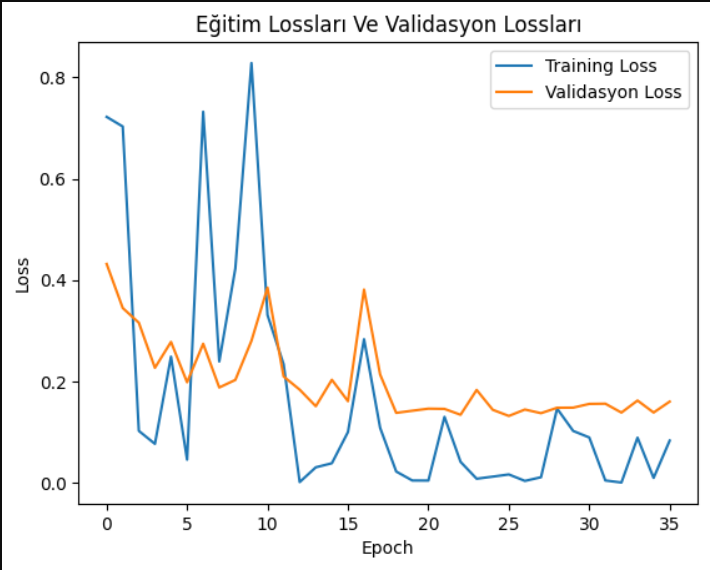
\includegraphics[width=0.75\textwidth]{train-validation-loss.png}
    \caption{Training ve Validation Loss Değerleri}
    \label{fig:my_pic}
\end{figure}

\begin{python}

torch.manual_seed(170401060)

# Eğitim döngüsü
epochs = 100
batch_size = 16
train_losses = [] # Eğitim losslarını saklamak için bir liste
val_losses = [] # Validasyon losslarını saklamak için bir liste

for epoch in range(epochs):
    # Batch'lerle veriyi yükle
    model.train() # Modeli eğitim modunda kullan
    train_loss = 0.0
    indices = torch.randperm(X_train.shape[0])
    for i in range(0, X_train.shape[0], batch_size):
        batch_indices = indices[i:i+batch_size]
        batch_X = X_train[batch_indices]
        batch_y = y_train[batch_indices]
        
        # Gradientleri sıfırla
        optimizer.zero_grad()
        
        # Forward pass
        y_pred = model(batch_X)
        
        # Loss hesapla
        loss = criterion(y_pred.squeeze(), batch_y)
        
        # Backward pass
        loss.backward()
        
        # Parametreleri güncelle
        optimizer.step()
        
        train_loss += loss.item() * batch_X.size(0)
        
    train_loss /= X_train.shape[0]
    train_losses.append(loss.item())
    
    # Her epoch sonunda kaybı yazdır
    print("Epoch [{}/{}], Loss: {:.4f}".format(epoch+1, epochs, loss.item()))
    

    # Modeli değerlendirme
    model.eval() 
    val_loss = 0.0
    with torch.no_grad():
        for i in range(0, X_val.shape[0], batch_size):
            batch_X = X_val[i:i+batch_size]
            batch_y = y_val[i:i+batch_size]
            y_pred = model(batch_X)
            loss = criterion(y_pred.squeeze(), batch_y)
            val_loss += loss.item() * batch_X.size(0)
        val_loss /= X_val.shape[0]
        val_losses.append(val_loss)
        
        # Validasyon Loss'unu yazdır.
        print("Epoch [{}/{}], Train Loss: {:.4f}, Val Loss: {:.4f}".format(epoch+1, epochs, train_loss, val_loss))
        
\end{python}



\subsection{(10 Puan)} \textbf{SEED=öğrenci numaranız set ettikten sonra altıncı haftada ödev olarak verdiğim gibi earlystopping'deki en iyi modeli kullanarak, Prensesi İyileştir test setinden accuracy, F1, precision ve recall değerlerini hesaplayan kodu yazın ve sonucu da aşağı yapıştırın. \%80'den fazla başarı bekliyorum test setinden. Daha düşükse başarı oranınız, nerede hata yaptığınızı bulmaya çalışın. \%90'dan fazla başarı almak mümkün (ben denedim).}

\begin{python}

# Test veri kümesinde doğruluk değerini hesapla
test_loss = 0.0
correct = 0
total = 0
with torch.no_grad():
    for i in range(0, X_test.shape[0], batch_size):
        batch_X = X_test[i:i+batch_size]
        batch_y = y_test[i:i+batch_size]
        y_pred = model(batch_X)
        loss = criterion(y_pred.squeeze(), batch_y)
        test_loss += loss.item() * batch_X.size(0)
        predicted = torch.round(y_pred).squeeze()
        correct += (predicted == batch_y).sum().item()
        total += batch_X.size(0)

test_loss /= X_test.shape[0]
accuracy = correct / total
print(f"Test accuracy: {accuracy:.4f}")
# Sonuçları ekrana yazdır
print(f"Toplam süre: {total_time:.2f} saniye")

# Tahminleri yap
with torch.no_grad():
    model.eval()
    y_pred = model(X_test)
    y_pred_classes = y_pred.argmax(dim=1)
    if y_test.ndim > 1:
        y_true = y_test.argmax(axis=1)
    else:
        y_true = y_test

# Confusion matrix'i hesapla
confusion_mtx = confusion_matrix(y_true, y_pred_classes)

# Hassasiyet (precision) hesapla
precision = precision_score(y_true, y_pred_classes, average='weighted', zero_division=1)

# Duyarlılık (recall) hesapla
recall = recall_score(y_true, y_pred_classes, average='weighted', zero_division=1)

# F1 değerini hesapla
f1 = 2 * (precision * recall) / (precision + recall)

# Sonuçları yazdır
print("Confusion Matrix:\n", confusion_mtx)
print("Precision: {:.4f}".format(precision))
print("Recall: {:.4f}".format(recall))
print("F1 Score: {:.4f}".format(f1))

\end{python}

Test accuracy: 0.9365
Confusion Matrix:
 [[384   0]
 [388   0]]
Precision: 0.7500
Recall: 0.4974
F1 Score: 0.5981

\subsection{(5 Puan)} \textbf{Tüm kodların CPU'da çalışması ne kadar sürüyor hesaplayın. Sonra to device yöntemini kullanarak modeli ve verileri GPU'ya atıp kodu bir de böyle çalıştırın ve ne kadar sürdüğünü hesaplayın. Süreleri aşağıdaki tabloya koyun. GPU için Google Colab ya da Kaggle'ı kullanabilirsiniz, iki ortam da her hafta saatlerce GPU hakkı veriyor.}

\begin{table}[ht!]
    \centering
    \caption{Calisma Sureleri}
    \begin{tabular}{c|c}
        Ortam & Süre (saniye) \\\hline
        CPU & Toplam süre: 2.95 saniye \\
        GPU & Toplam süre: 3.80 saniye\\
    \end{tabular}
    \label{tab:my_table}
\end{table}

\subsection{(3 Puan)} \textbf{Modelin eğitim setine overfit etmesi için elinizden geldiği kadar kodu gereken şekilde değiştirin, validasyon loss'unun açıkça yükselmeye başladığı, training ve validation loss'ları içeren figürü aşağı koyun ve overfit için yaptığınız değişiklikleri aşağı yazın. Overfit, tam bir çanak gibi olmalı ve yükselmeli. Ona göre parametrelerle oynayın.}

\begin{figure}[ht!]
    \centering
    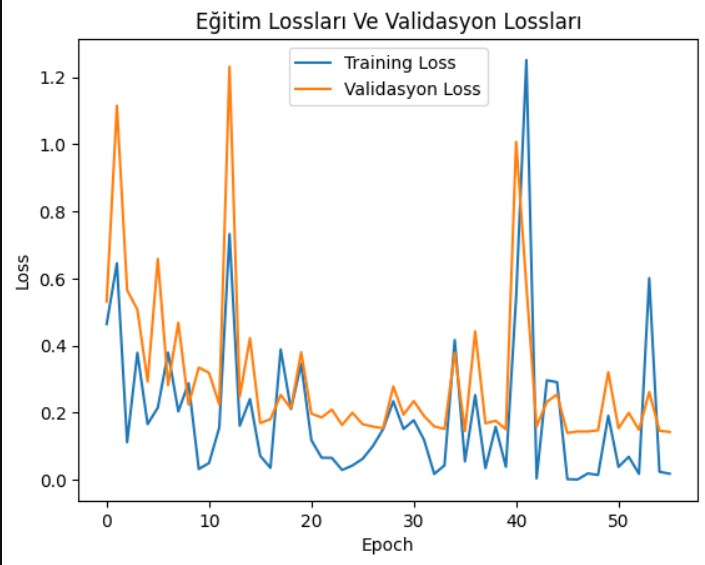
\includegraphics[width=0.75\textwidth]{overfitting-loss.png}
    \caption{Overift etmiş hali}
    \label{fig:my_pic}
\end{figure}

Modelin overfit edebilmesi için batch size'ı 32 yaptım. 
Validasyon loss değeri artmaya başladı.

% Figür aşağı
% Hocam 5.5 sorusunun figürü burada. 
% Template yüzünden aşağısına koyamadım. 
% Resimi aşağı kısma koyunca kayıyor ve 6. soruyla karışıyor.


\subsection{(2 Puan)} \textbf{Beşinci soruya ait tüm kodların ve cevapların olduğu jupyter notebook'un Github linkini aşağıdaki url'e koyun.}

\url{https://github.com/UmutcanCerlet604/neural_networks_2.git}

\section{(Toplam 10 Puan)} \textbf{Bir önceki sorudaki Prensesi İyileştir problemindeki yapay sinir ağınıza seçtiğiniz herhangi iki farklı regülarizasyon yöntemi ekleyin ve aşağıdaki soruları cevaplayın.} 

\subsection{(2 puan)} \textbf{Kodlarda regülarizasyon eklediğiniz kısımları aşağı koyun:} 

\begin{python}
# MLP modelini tanimla
class MLP(nn.Module):
    def __init__(self):
        super(MLP, self).__init__()
        self.fc1 = nn.Linear(13, 100)
        self.fc2 = nn.Linear(100, 50)
        self.fc3 = nn.Linear(50, 1)
        self.relu = nn.ReLU()
        self.sigmoid = nn.Sigmoid()
        self.dropout = nn.Dropout(0.2)
        
    def forward(self, x):
        x = self.fc1(x)
        x = self.relu(x)
        x = self.dropout(x)
        x = self.fc2(x)
        x = self.relu(x)
        x = self.dropout(x)
        x = self.fc3(x)
        x = self.sigmoid(x)
        return x
\end{python}

\begin{python}
    # Early stopping icin degiskenleri tanimla
    best_val_loss = float('inf')
    best_epoch = 0
    patience = 10
    current_patience = 0

    # Early stopping kontrolü
        if val_loss < best_val_loss:
            best_val_loss = val_loss
            best_epoch = epoch
            current_patience = 0
        else:
            current_patience += 1
        
        if current_patience == patience:
            print(f"Early stopping triggered at epoch {epoch}, best validation loss: {best_val_loss:.4f}")
            break
\end{python}

\begin{python}
    optimizer = optim.SGD(model.parameters(), lr=0.01, weight_decay=0.01)
    # Ridge regularizasyonunu ekledik, weight_decay parametresi ile regularizasyon katsayisini ayarladik.
\end{python}

\begin{python}
    optimizer = optim.SGD(model.parameters(), lr=0.01, weight_decay=0.01, momentum=0.9)
    # Elastic Net regularizasyonunu ekledik, weight_decay parametresi ile regularizasyon katsayisini ayarladik.
\end{python}

\subsection{(2 puan)} \textbf{Test setinden yeni accuracy, F1, precision ve recall değerlerini hesaplayıp aşağı koyun:}

Sadece early stopping uygulandığında;
Early stopping triggered at epoch 62, best validation loss: 0.1250
Test accuracy: 0.9521
Toplam süre: 4.63 saniye
Confusion Matrix:
 [[384   0]
 [388   0]]
Precision: 0.7500
Recall: 0.4974
F1 Score: 0.5981

Ridge uygulandığında sonuçlar;
Early stopping triggered at epoch 97, best validation loss: 0.1051
Test accuracy: 0.9534
Toplam süre: 7.17 saniye
Confusion Matrix:
 [[384   0]
 [388   0]]
Precision: 0.7500
Recall: 0.4974
F1 Score: 0.5981

Elastic Net uygulandığında sonuçlar;
Early stopping triggered at epoch 25, best validation loss: 0.1859
Test accuracy: 0.8964
Toplam süre: 2.28 saniye
Confusion Matrix:
 [[384   0]
 [388   0]]
Precision: 0.7500
Recall: 0.4974
F1 Score: 0.5981

\subsection{(5 puan)} \textbf{Regülarizasyon yöntemi seçimlerinizin sebeplerini ve sonuçlara etkisini yorumlayın:}

Ridge uygulanıp sonuçlara bakıldığında test accuracy değerinin çok az da olsa bir artış gösterdiğini görebiliyoruz.
Modelim zaten yüksek bir test doğruluk değerine sahip ve Ridge regülarizasyonunu eklediğimde doğruluk değeri arttığı için, bu regülarizasyonun modelimin karmaşıklığını azaltarak genelleştirme performansını artırdığını ve aşırı uydurma riskini azalttığını söyleyebilirim. Ridge regülarizasyonu, ağırlıkları sıfıra yakın değerlere çekerek modelin düzenlenmesini sağlıyor, ancak tamamen sıfırlamıyor. Bu nedenle modelin tahmin yeteneğini etkilemeden aşırı uydurma riskini azalttığını düşünüyorum.


Elastic Net uygulanıp sonuçlara bakıldığında test accuracy değerinde bir düşüş görebiliyoruz.
Elastic Net regülarizasyonunu modele eklediğimde, test doğruluk değerinin düşmesi, modelin genelleştirme yeteneğinin azaldığını ve aşırı uydurma (overfitting) yapma eğiliminin arttığını gösteriyor.Ancak, Elastic Net regülarizasyonu, ağırlık değerlerini sınırlayarak modelin karmaşıklığını azalttığından, modelin doğru sonuçları tahmin etme yeteneğini de etkileyebilmesi olası bir durumdur.Modelin iyi bir doğruluk değerine sahip olduğunu düşünüyorum. Regülarizasyonu eklediğimde doğruluk değerinin düşmesinin nedenini modelin karmaşıklığını fazla düşürdüğü veya aşırı düzenleme (over-regularization) yaptığına bağlıyorum. 

İki farklı regülarizasyon yöntemi kullandığımda da F1, precision ve recall değerleri hiç değişmedi.
Regülarizasyon yöntemlerinin etkisi, kullanılan regülarizasyon türüne, regülarizasyon katsayılarına ve veri setine bağlıdır. Modelimin aşırı uydurma riski düşük bir seviyede olduğunu düşünüyorum. Bu yüzden regülarizasyon yöntemlerini eklemenin performans üzerinde belirgin bir etkisi olmama ihtimalini aklıma geliyor. Tam olarak bu sebepten ötürü bir değişim görmediğimizi düşünüyorum.

\subsection{(1 puan)} \textbf{Sonucun github linkini  aşağıya koyun:}

\url{https://github.com/UmutcanCerlet604/neural_networks_2_1.git}

\end{document}